Dieser Versuch befasst sich mit der Messung der Wirk- und Blindleistung mithilfe eines Multiplikators und eines trägen Messgerätes. Es wird zusätzlich die Scheinleistung berechnet, und die berechneten und gemessenen Ergebnisse werden miteinander verglichen.

\subsubsection{Versuchsaufbau}

Der Versuchsaufbau ähnelt weitestgehend dem in Abschnitt \ref{sec:Aufbau2.2.1} beschriebenen. Es wird jedoch das Oszilloskop durch einen Multiplikator und ein träges, analoges Messgerät gemäß Abbildung \ref{fig:Plan2-2} ersetzt. Das Messgerät wird auf Gleichspannung eingestellt und misst somit den Gleichanteil der Spannung $u_P(t)$, welche durch die Multiplikation von Spannung $u_U(t)$ und zum Strom proportionalen Spannung $u_I(t)$ eine zur Momentanleistung proportionale Größe dar stellt. Somit kann nach Bestimmung des Proportionalitätsfaktors die Wirkleistung gemessen werden.

\begin{figure}[H]
\centering
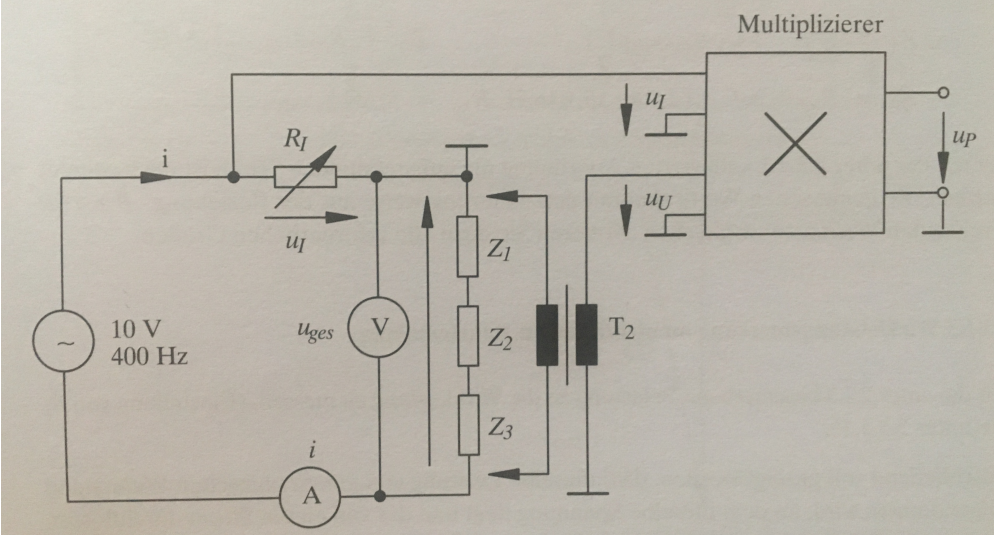
\includegraphics[width=0.7\linewidth]{Images/Aufbau2-2.png}
\caption{Schaltplan eines Versuches zur Messung der Wirkleistung eines Schaltkreises}
\label{fig:Plan2-2}
\end{figure}
Die Impedanzen $Z_1$ bis $Z_3$ werden je nach zu messender Größe verändert.

\subsubsection{Kalibrierung des Drehspulmessinstrumentes}
Damit die Wirkleistung aus den am Messgerät abgelesenen Werten errechnet werden kann, muss die Proportionalitätskonstante, im Folgenden "K", sowie der Offset des Multiplizierers bestimmt werden.
Es gilt:
\begin{equation}
K\cdot \overline{u_P(t)} = P
\label{eq:PropFaktor}
\end{equation}

Der Offset wird gemessen indem die Anschlüsse des potentialtrennenden Transformators kurzgeschlossen werden. $u_U(t)=0$ gilt nun, d.h. das Messgerät sollte null anzeigen.
Angezeigt wird jedoch ein Wert von $-1mV$, d.h. die gemessenen Werte müssen um $1mV$ korrigiert werden. Alle im Folgenden aufgeführten Messwerte wurden um diesen Faktor bereits korrigiert.

Es wird $Z_1 = 40\Omega; Z_2 = Z_3 = 0\Omega$ eingebaut. $u_{ges}$ wird durch Veränderung von $R_I$ auf 6V eingestellt. $I$ wird hierbei als $0.16A$ gemessen. Durch eine Phasenverschiebung von $\varphi = 0$ am ohm'schen Verbraucher lässt sich nun die Wirkleistung entsprechend \eqref{eq:LeistungGleichanteil} berechnen als:
\begin{equation*}
P_{mes}=U_{ges}I = 6V\cdot 0.16A = 0.96W
\end{equation*}
Das Messgerät zeigt eine Spannung von $\overline{u_P}=0.475V$ an. 
Durch Umstellen von Gleichung \eqref{eq:PropFaktor} lässt sich nun der Proportionalitätsfaktor bestimmen:
\begin{equation*}
K=\frac{P_{mes}}{\overline{u_P}} = \frac{0.96W}{0.475V} = 2.021A
\end{equation*}

\subsubsection{Messung der Wirkleistung}

Dieser Versuchsteil befasst sich mit der Messung der Wirkleistung, welche von verschiedenen Verbrauchern aufgenommen wird. Der Versuchsaufbau gleicht dem vorherigen Versuchsteil, bis auf die Impedanzen. Für sie gilt nun:
\begin{itemize}
\item $Z_1 = \frac{1}{j\omega C} \mbox{ mit } C = 6\mu F$
\item $Z_2 = [30; 40; \cdots; 80]\Omega$
\item $Z_3 = R_{sp} + j\omega L \mbox{ mit } L = 15.84mH; R_{sp} = 5.5\Omega$
\end{itemize}
$R_I$ darf hierbei nicht mehr verändert werden. Grund dafür ist, dass die Spannung $u_I$, welche zur Berechnung von $u_P$ und somit der Wirkleistung verwendet wird, von $R_I$ abhängt.
Im Folgenden wird $Z_2$ variiert. Die Spannung $\overline{u_P}$ wird abgelesen und mit Gleichung \eqref{eq:PropFaktor} die Wirkleistung berechnet. Zusätzlich werden $U_{ges}$ und $I$ an den Messgeräten abgelesen. Zum Vergleich wird die Wirkleistung mit Formel \eqref{eq:KomplexP} und der komplexen Impedanz $Z_{ges}$ berechnet.
\\
Folgende Messwerte wurden aufgenommen:

\begin{large}
\begin{center}
\begin{tabular}{| c | c | c | c | c | c |}
\hline
$\frac{Z_2}{\Omega}$ & $\frac{\overline{u_P}}{V}$ 
& $\frac{P_{mes}}{W}$ & $\frac{P_{calc}}{W}$ & $\frac{U_{ges}}{V}$ & $\frac{I_{ges}}{A}$\\
\hline

30 & 0.374 & 0.759 & 0.696 & 6.8 & 0.14 \\
40 & 0.384 & 0.780 & 0.768 & 7.2 & 0.13 \\
50 & 0.384 & 0.780 & 0.740 & 7.5 & 0.12 \\
60 & 0.384 & 0.780 & 0.722 & 7.7 & 0.11 \\
70 & 0.364 & 0.739 & 0.696 & 8   & 0.10 \\
80 & 0.340 & 0.709 & 0.693 & 8.2 & 0.09 \\
\hline
\end{tabular}
\end{center}
\end{large}

Zu erkennen ist eine relativ genaue Übereinstimmung der gemessenen Werte mit den berechneten. Ungenauigkeiten beim Ablesen der analogen Skala am Messgerät erklären die konstanten Werte zwischen $Z_2 = 40\Omega$ und $60\Omega$, weitere Abweichungen von den berechneten Werten können durch Messfehler bei der Bestimmung des Faktors K und dem Offset entstehen. Auch ist es möglich, dass $Z_1 \mbox{ bis } Z_2$ nicht die angegebenen Werte besitzen, d.h. die berechnete Wirkleistung kann auch fehlerbehaftet sein.

\subsubsection{Messung der Blindleistung}
Dieser Versuchsteil befasst sich mit der Messung der Blindleistung der bereits im vorherigen Abschnitt verwendeten Impedanzen. Anhand der Formel \eqref{eq:ScheinleistungPythagoras} werden zusätzlich die Messergebnisse miteinander verglichen.

Um die Blindleistung mit möglichst wenig Aufwand, d.h. hier mit möglichst wenig Modifikation an der vorliegenden Schaltung messen zu können, wird wie in Abschnitt \ref{sec:MessungBlindleistung} erläutert ein Kondensator in den Spannungspfad des Messgerätes eingebaut, um dessen Phase um $90^\circ$ zu drehen. Hiermit gibt der Gleichanteil der Spannung $u_P$ die Blindleistung, nicht mehr die Wirkleistung, an.

Es wird ein Kondensator von $C=2nF$ direkt hinter $T_2$ geschaltet. Dessen Größe wurde so bemessen, dass eine Phasenverschiebung von ca. $84^\circ$ möglich ist, ohne dass das Spannungssignal zu klein wird. $u_U$ ist nun durch die Impedanz des Kondensators etwa 10 mal kleiner, der Kalibrierungsfaktor $K$ muss dementsprechend angepasst werden. Es gilt jetzt:
\begin{equation*}
K_{Q} = 10\cdot K = 20.21A
\end{equation*}

Für die gleichen Impedanzen wie zuvor werden nun die Spannungen $\overline{u_P}$ gemessen und die Blindleistungen berechnet. Gesamtströme und -spannungen sind aus den vorherigen Messungen bekannt. Die anhand von Formel \eqref{eq:KomplexQ} berechnete Blindleistung wird zum Vergleich aufgeschrieben.

\begin{large}
\begin{center}
\begin{tabular}{| c | c | c | c |}
\hline
$\frac{Z_2}{\Omega}$ & $\frac{\overline{u_P}}{V}$ & 
$\left|\frac{Q_{mes}}{var}\right|$ & $\left|\frac{Q_{calc}}{var}\right|$ \\
\hline
30 & 0.022 & 0.485 & 0.520 \\
40 & 0.017 & 0.384 & 0.449 \\
50 & 0.013 & 0.303 & 0.354 \\
60 & 0.010 & 0.243 & 0.293 \\
70 & 0.008 & 0.202 & 0.245 \\
80 & 0.006 & 0.162 & 0.215 \\
\hline
\end{tabular}
\end{center}
\end{large}

Auch hier sieht man eine gute Übereinstimmung der Messwerte mit den berechneten Werten. Diskrepanzen lassen sich wie zuvor durch ein falsch bestimmtes K, Ablese- und Messfehler erklären. Einzubeziehen ist auch, dass die Phasenverschiebung nur ca. $84^\circ$ beträgt, und der genaue Wert des Kondensators nicht exakt $2nF$ sein muss.

Schlussendlich lassen sich nun die Messwerte anhand von Formel \eqref{eq:ScheinleistungPythagoras} miteinander Vergleichen. $S_1$ wird hierbei mit der Beziehung $S=U\cdot I$ berechnet, $S_2$ anhand von Formel \eqref{eq:ScheinleistungPythagoras}

\begin{large}
\begin{center}
\begin{tabular}{| c | c | c |}
\hline
$\frac{S_1}{VA}$ & $\frac{S_2}{VA}$ & $\frac{S_2}{S_1}$ \\
\hline
0.952 & 0.902 & 0.947 \\
0.936 & 0.870 & 0.929 \\
0.866 & 0.837 & 0.966 \\
0.809 & 0.817 & 1.010 \\
0.768 & 0.767 & 0.998 \\
0.738 & 0.728 & 0.986 \\
\hline
\end{tabular}
\end{center}
\end{large}